\chapter{Waar dieren wonen}\label{ch:g2:where-animals-live}

Je komt geen forel tegen op het schoolplein, en geen eekhoorn op de
bodem van de vijver. Elk \omterm{def:g1:animals-around-us:animal}{dier} woont op het soort plek dat bij hem past
--- waar hij zijn voedsel, zijn schuilplaats en zijn buren vindt.
Biologen hebben een naam voor het thuisgebied van een \omterm{def:g1:animals-around-us:animal}{dier}.

\section{Leefgebieden}

\begin{definition}[Leefgebied]\label{def:g2:where-animals-live:habitat}
Het \emph{leefgebied}\index{leefgebied} van een \omterm{def:g1:animals-around-us:animal}{dier} is het soort plek
waar het van nature woont en alles vindt wat het nodig heeft: voedsel,
water, schuilplaats en een veilig plekje voor zijn jongen. De vijver,
het bos, de wei, de heg en het strand zijn leefgebieden.
\end{definition}

\begin{example}[Vier leefgebieden, vier buurten]\label{ex:g2:where-animals-live:four}
In de \emph{vijver}: kikkers, libellen, stekelbaarsjes,
poelslakken. In het \emph{bos}: eekhoorns, herten, spechten, bosmieren.
In de \emph{wei}: konijnen, sprinkhanen, vlinders, veldmuizen. Onder de
stenen van een oude \emph{muur}: pissebedden, spinnen, en soms een
hagedis die er bovenop ligt te zonnen.
\end{example}

\begin{omfigure}
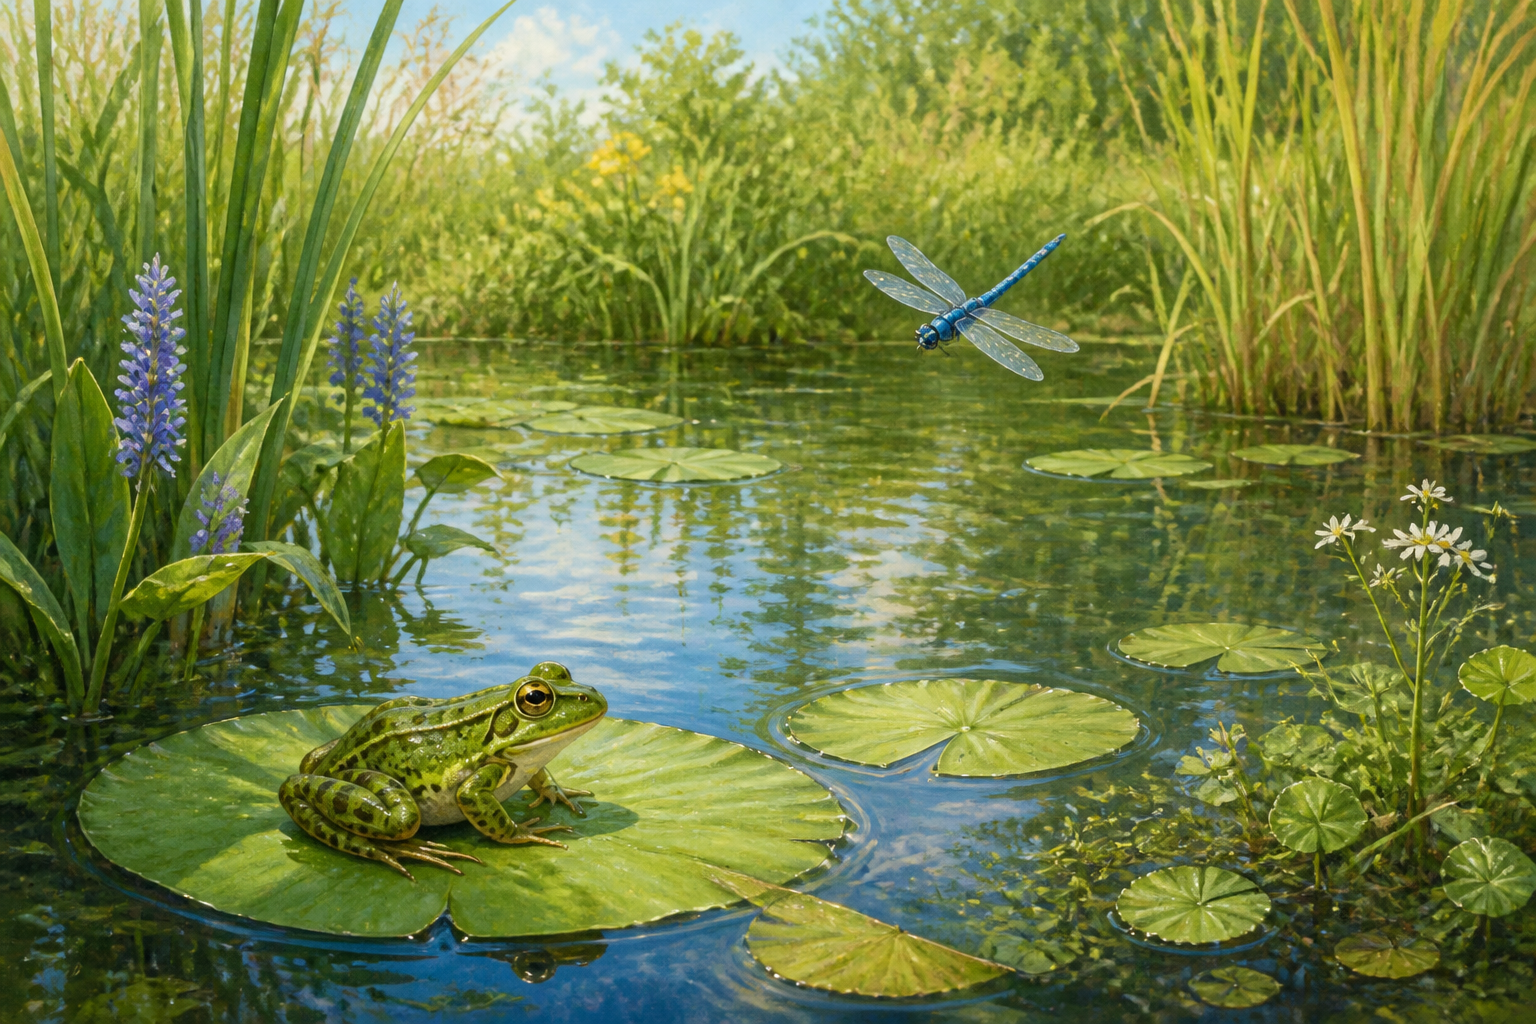
\includegraphics[width=0.62\linewidth]{images/book1/ai/g2-live-pond.png}

{\small Het \omterm{def:g2:where-animals-live:habitat}{leefgebied} van de vijver met twee van zijn bewoners thuis:
een kikker op een waterlelieblad, een libel op patrouille.}
\end{omfigure}

\begin{omfigure}
\begin{tikzpicture}[scale=0.88]
  \draw[thick, omDef, fill=omDef!7, rounded corners=6pt]
    (0,0) rectangle (3.4,2.6);
  \draw[thick, omMeth, fill=omMeth!7, rounded corners=6pt]
    (3.9,0) rectangle (7.3,2.6);
  \draw[thick, omProp, fill=omProp!7, rounded corners=6pt]
    (7.8,0) rectangle (11.2,2.6);
  \node[font=\small\bfseries, omDef] at (1.7,2.25) {de vijver};
  \node[font=\small\bfseries, omMeth] at (5.6,2.25) {het bos};
  \node[font=\small\bfseries, omProp] at (9.5,2.25) {de wei};
  \node[font=\small, align=center] at (1.7,1.05)
    {kikker\\ libel\\ stekelbaars};
  \node[font=\small, align=center] at (5.6,1.05)
    {eekhoorn\\ specht\\ hert};
  \node[font=\small, align=center] at (9.5,1.05)
    {konijn\\ sprinkhaan\\ vlinder};
\end{tikzpicture}

{\small Drie \omterm{def:g2:where-animals-live:habitat}{leefgebieden} en een paar van hun bewoners. Probeer ze eens
te verwisselen --- de eekhoorn zou het in de vijver niet lang uithouden.}
\end{omfigure}

\begin{remark}[Eén leefgebied, veel woningen]\label{rem:g2:where-animals-live:layers}
Een \omterm{def:g2:where-animals-live:habitat}{leefgebied} heeft veel hoekjes. In hetzelfde bos woont de specht
hoog op de stammen, de eekhoorn in de takken, het hert tussen de
struiken, en de bosmieren op de grond in hun opgehoopte nest. Hetzelfde
bos, verschillende verdiepingen --- zo kunnen veel \omterm{def:g1:animals-around-us:animal}{dieren} één
\omterm{def:g2:where-animals-live:habitat}{leefgebied} delen zonder dat het te vol wordt.
\end{remark}

\section{Passend bij het leefgebied}

\begin{proposition}[Dieren passen bij hun leefgebied]\label{prop:g2:where-animals-live:fit}
Het lichaam en de gewoonten van een \omterm{def:g1:animals-around-us:animal}{dier} passen bij de plek waar het
woont:
\begin{itemize}
  \item de zwemvliezen van de kikker duwen het water weg --- gemaakt
        voor de vijver;
  \item de grijpende klauwen en de grote balanceerstaart van de
        eekhoorn zijn gemaakt voor bomen;
  \item de gravende poten en de lange waarschuwingsoren van het konijn
        zijn gemaakt voor de open wei met holen eronder;
  \item de \omterm{def:g1:animals-around-us:covering}{veren} van de eend laten het water aflopen, en zijn
        zwemvliezen peddelen.
\end{itemize}
In het verkeerde \omterm{def:g2:where-animals-live:habitat}{leefgebied} verliest een \omterm{def:g1:animals-around-us:animal}{dier} al deze voordelen.
\end{proposition}
\admitted

\begin{example}[De uitrusting van de mol]\label{ex:g2:where-animals-live:mole}
De mol woont ondergronds, in gangen die hij onder de wei graaft. Zijn
handen zijn brede graafschoppen, zijn \omterm{def:g1:animals-around-us:covering}{vacht} ligt in beide richtingen
glad zodat de aarde hem nooit in de war maakt, en zijn zwakke \omterm{def:g1:the-five-senses:sense}{ogen} doen
er in het donker nauwelijks toe. Boven de grond is hij onhandig; in
zijn eigen \omterm{def:g2:where-animals-live:habitat}{leefgebied} is hij een kampioen.
\end{example}

\begin{method}[Een dier bij zijn leefgebied zoeken]\label{met:g2:where-animals-live:matching}
Bij een onbekend \omterm{def:g1:animals-around-us:animal}{dier}:
\begin{enumerate}
  \item kijk naar zijn uitrusting: zwemvliezen? klauwen? vleugels?
        graafpoten?
  \item vraag wat het eet, en waar dat voedsel te vinden is;
  \item vraag waar het kan schuilen en jongen kan grootbrengen;
  \item het \omterm{def:g2:where-animals-live:habitat}{leefgebied} dat op alle drie antwoord geeft, is
        waarschijnlijk zijn thuis.
\end{enumerate}
\end{method}

\section{Leefgebieden kunnen verdwijnen}

\begin{proposition}[Geen leefgebied, geen bewoners]\label{prop:g2:where-animals-live:loss}
Een \omterm{def:g1:animals-around-us:animal}{dier} kan niet leven zonder zijn \omterm{def:g2:where-animals-live:habitat}{leefgebied}. Als een vijver gedempt
wordt, verdwijnen zijn kikkers en libellen ermee; als een heg wordt
uitgerukt, raken de vogels die er nestelden hun schuilplaats kwijt.
\omterm{def:g1:animals-around-us:animal}{Dieren} beschermen begint bij het beschermen van de plekken waar ze wonen.
\end{proposition}
\admitted

\begin{example}[De schoolvijver]\label{ex:g2:where-animals-live:schoolpond}
Een school graaft een vijvertje in een hoek van het plein. Binnen twee
jaar patrouilleren er libellen, lopen er schaatsenrijders op het water
en hebben kikkers er hun intrek genomen --- niemand heeft ze gebracht.
Maak het \omterm{def:g2:where-animals-live:habitat}{leefgebied}, en de bewoners vinden het.
\end{example}

\begin{remark}[Kijken zonder te storen]\label{rem:g2:where-animals-live:respect}
Als we een \omterm{def:g2:where-animals-live:habitat}{leefgebied} bezoeken, zijn we gasten. Kijk stil toe, leg
stenen terug zoals je ze vond, laat eieren en nesten met rust, en neem
je afval mee naar huis --- het \omterm{def:g2:where-animals-live:habitat}{leefgebied} hoort te vergeten dat je er
geweest bent. De volgende hoofdstukken geven meer manieren om voor de
natuur te zorgen.
\end{remark}

\section{Oefeningen}

\begin{exercise}[$\star$]\label{exo:g2:where-animals-live:1}
Wat is een \omterm{def:g2:where-animals-live:habitat}{leefgebied}? Noem de vier dingen die een \omterm{def:g1:animals-around-us:animal}{dier} erin vindt.
\end{exercise}

\begin{exercise}[$\star$]\label{exo:g2:where-animals-live:2}
Geef twee \omterm{def:g1:animals-around-us:animal}{dieren} van de vijver, twee van het bos en twee van de wei.
\end{exercise}

\begin{exercise}[$\star$]\label{exo:g2:where-animals-live:3}
Welk \omterm{def:g2:where-animals-live:habitat}{leefgebied} past bij elk \omterm{def:g1:animals-around-us:animal}{dier}: de stekelbaars, de specht, de
sprinkhaan, de pissebed?
\end{exercise}

\begin{exercise}[$\star$]\label{exo:g2:where-animals-live:4}
Wat is de zwemuitrusting van de kikker? En de klimuitrusting van de
eekhoorn?
\end{exercise}

\begin{exercise}[$\star$]\label{exo:g2:where-animals-live:5}
Noem de drie stukken ondergrondse uitrusting van de mol uit
\cref{ex:g2:where-animals-live:mole}.
\end{exercise}

\begin{exercise}[$\star$]\label{exo:g2:where-animals-live:6}
Welke ``verdieping'' van het bos gebruikt elk \omterm{def:g1:animals-around-us:animal}{dier} in
\cref{rem:g2:where-animals-live:layers}: specht, eekhoorn, hert,
bosmier?
\end{exercise}

\begin{exercise}[$\star$]\label{exo:g2:where-animals-live:7}
Wat gebeurt er met de kikkers en libellen als een vijver gedempt wordt?
Wat leert dat over het beschermen van \omterm{def:g1:animals-around-us:animal}{dieren}?
\end{exercise}

\begin{exercise}[$\star$]\label{exo:g2:where-animals-live:8}
Probeer het: kies één klein \omterm{def:g2:where-animals-live:habitat}{leefgebied} bij jou in de buurt --- onder
een steen, een struik, een bloemperk. Kijk stil toe en noteer elk \omterm{def:g1:animals-around-us:animal}{dier}
dat je in een vaste tijd ziet. Leg elke steen terug. Hoeveel bewoners
had jouw kleine \omterm{def:g2:where-animals-live:habitat}{leefgebied}?
\end{exercise}

\begin{exercise}[$\star\star$]\label{exo:g2:where-animals-live:9}
Een raadseldier heeft zwemvliezen, dichte \omterm{def:g1:animals-around-us:covering}{veren} die het water laten
aflopen, en een platte snavel om mee te zeven. Gebruik
\cref{met:g2:where-animals-live:matching} om zijn \omterm{def:g2:where-animals-live:habitat}{leefgebied} te noemen
--- en misschien ook het \omterm{def:g1:animals-around-us:animal}{dier}.
\end{exercise}

\begin{exercise}[$\star\star$]\label{exo:g2:where-animals-live:10}
Tom wil een kikker ``helpen'' door hem mee naar huis te nemen naar een
droog terrarium met volop voedsel. Leg met
\cref{prop:g2:where-animals-live:fit} en
\cref{prop:g2:where-animals-live:loss} uit waarom dat de kikker
helemaal niet zou helpen.
\end{exercise}
